\chapter{Distribution And Fusion Case Study}
\label{chap:ch4}

In this chapter, we will discuss about a case study done on Frontier Pass which we have develop for our proposed Machine Learning (ML) based Loop Distribution. In section \ref{sec:distribution:bg}, background to Loop Distribution and it's benefits. In section \ref{sec:distribution:intro}, our proposed solution and it's components. In section \ref{sec:distribution:fp}, details of Frontier Pass which we have implemented. In section \ref{sec:distribution:ideo} and \ref{sec:distribution:case}, importance of  Frontier Pass and and results to substantiate it. In section~\ref{sec:distribution:conclusion}, we will conclude this chapter.


\section{Background}\label{sec:distribution:bg}
    The optimization in the compiler is very important of code generation.
Good optimization lead to faster execution of the program. Here, we will talk about Loop Distribution optimization.

    In Loop Distribution, the bigger loop is split into smaller loops as shown in Fig.~\ref{fig:dist-introduction}. It may lead to improved loop vectorization and better locality. In LLVM~\cite{Lattner:2004:llvm}, the loop distribution is not efficient, heuristic-based and does not promise the optimal distribution. It lead to miss in the vectorization opportunities.

\begin{figure}[t]
    \centering
    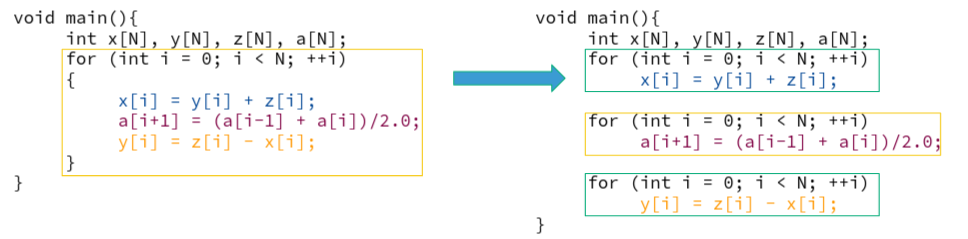
\includegraphics[scale=0.45]{figures/chapter-4/distribution_introduction.png}
    \caption{Distributed Loops}
     \label{fig:dist-introduction}
\end{figure}

\section{Introduction}\label{sec:distribution:intro}
We want to have a ML based Loop Distribution optimization in the LLVM's pipeline. It could overcome the flaws of the existing Loop Distribution. But in this chapter, we will discuss about Frontier Pass and it's importance.

\begin{figure}[t]
    \centering
    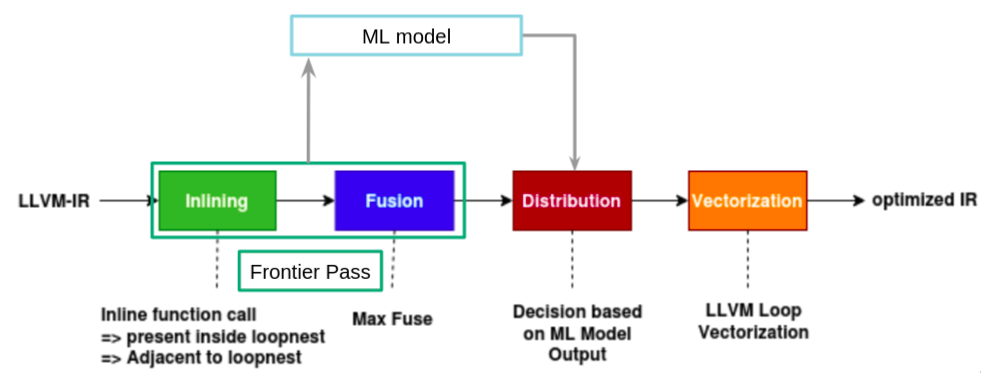
\includegraphics[scale=0.4]{figures/chapter-4/distribution_flow.png}
    \caption{Position of Frontier Pass in the workflow}
     \label{fig:dist-flow}
\end{figure}

\section{Frontier Pass}\label{sec:distribution:fp}
 We have proposed a pass sequence of custom inlining followed by fusion. See the Fig.~\ref{fig:dist-flow}. We have written loop-function-inline pass, which pass through loop and try to forcefully inline the function inside the innermost loop as well as at the same level of the loop. After performing loop-function inlining, we have enable the fusion pass in the pipeline. The loop fusion is the reverse of loop distribution. The fusion combined multiple loop to form a big loop. 
 
%  The selected loop should not have any control flow  and call instruction inside it.


%  For the Bigger picture to happen, we have a design proposal that only innermost loop will be selected.

\section{Ideology Behind Frontier Pass}\label{sec:distribution:ideo}
To achieve the optimal distribution, we first want to have max distribution. The max distribution can be achieve from max fusion. As per the sec~\ref{sec:distribution:fp}, we have added fusion to the pipeline. For better fusion opportunities, some custom inlining can be helpful. We have developed loop-function-inline as mentioned in Sec.~\ref{sec:distribution:fp} and schedule it in the LLVM pass sequence. 

\begin{table}[h]
\begin{tabular}{|l|l|l|}
\hline
\multirow{2}{*}{\textbf{BENCHMARK}} & \multicolumn{2}{c|}{\textbf{\#Candidates for Loop Fusion}} \\ \cline{2-3} 
 & \textbf{O3-Fusion} & \textbf{O3-Frontier Pass} \\ \hline
blender\_r & 3952 & 7042 \\ \hline
deepsjeng\_r & 94 & 244 \\ \hline
imagick\_r & 2735 & 3065 \\ \hline
lbm\_r & 8 & 8 \\ \hline
leela\_r & 53 & 69 \\ \hline
mcf\_r & 14 & 16 \\ \hline
namd\_r & 1392 & 1812 \\ \hline
omnetpp\_r & 203 & 2200 \\ \hline
povray\_r & 229 & 2232 \\ \hline
x264\_r & 356 & 760 \\ \hline
xalancbmk\_r & 1017 & 1147 \\ \hline
xz\_r & 67 & 85 \\ \hline
\end{tabular}
\centering
\caption{Candidates for Loop Fusion}
\label{tab:dist:fuscand}
\end{table}

\section{Case Study}\label{sec:distribution:case}
In this section, we will see the effect of the frontier pass on the fusion candidates and runtime. We have run our xperimentation on the SPEC 2017 benchmark and  observe the fusion candidate. Here, we are comparing the metrics between the O3 optimization with fusion enabled and O3 optimization with Frontier Pass.

\subsection{Fusion Candidate}
Here, we are comparing the \# Candidates for Loop Fusion between the O3 optimization with fusion enabled and O3 optimization with Frontier Pass. See the Tab.~\ref{tab:dist:fuscand}. Incase of Frontier Pass, there are more fusion candidates which are better for max fusion. Hence frontier pass is important part of the ML-based loop distribution as the prepossessing step. 

\subsection{Runtime}
Here, we are comparing the runtime between the O3 optimization with fusion enabled and O3 optimization with Frontier Pass. See the Tab.~\ref{tab:dist:fpruntime}. Due to Frontier Pass,  they is not much overhead added to the runtime and they are some positive cases where there is improvement in runtime.



% Please add the following required packages to your document preamble:
% \usepackage{multirow}
\begin{table}[h]
\begin{tabular}{|l|l|l|}
\hline
\multirow{2}{*}{\textbf{BENCHMARK}} & \multicolumn{2}{c|}{\textbf{Runtime in seconds}} \\ \cline{2-3} 
 & \textbf{O3-Fusion} & \textbf{O3-Frontier Pass} \\ \hline
blender\_r & 298 & 311 \\ \hline
deepsjeng\_r & 343 & 336 \\ \hline
imagick\_r & 440 & 437 \\ \hline
lbm\_r & 544 & 545 \\ \hline
leela\_r & 503 & 498 \\ \hline
mcf\_r & 542 & 530 \\ \hline
namd\_r & 234 & 239 \\ \hline
omnetpp\_r & 636 & 602 \\ \hline
povray\_r & 459 & 439 \\ \hline
x264\_r & 422 & 284 \\ \hline
xalancbmk\_r & 407 & 392 \\ \hline
xz\_r & 303 & 442 \\ \hline
\end{tabular}
\centering
\caption{Runtime Overhead}
\label{tab:dist:fpruntime}
\end{table}

% \section{Model}
%  The generated graphs are used as inputs in our modeling pipeline. In this section, we explain how we represent SDGs using IR2Vec representations and the way we model the reinforcement learning model to consume this information using Gated Graph Neural Networks. We also discuss various parameters of the model, including the design of our cost model, with which we arrive at a relative number of clock ticks that take into account impact by both locality and vectorization.

% % CONSTRAINTS ON SDG
% % TOPOLOGICAL MATH FORMULATION
% % MERGE AND DISTRIBUTE

% \subsection{GGNN based reinforcement learning model}
%     Fig. 2 shows the workflow of the reinforcement learning model for our problem. The model takes SDG as input and maps it to a GGNN. The IR2Vec embeddings take the type of operation, a variable is involved into consideration.

%     GGNN[Y Li] is the upgradation of the graph neural network by adding an Gating mechanism using the Gated Recurrent Units  and unroll the recurrence
% for a fixed number of steps T. Each node of the GGNN has a hidden presentation which is initially represented using IR2Vec embeddings and dannotation vectors. 

% In our work, we use the propagation model of the GGNN to get the updated hidden state vectors at any instance of time, 

% Initial Presentation 
% hno = IR2vec Embedding according to SDG node   
% Hn0 : [hno:Ano]  
% A is the meta vector [isStartNode, IsVisited]
% Ano  = [0,0]  as no node visited in the starting

% At any instant t for node n
% Hnt-1 : [hnt-1:Ant-1]
% f : Hnt-1 → hant-1 
% % x :  ∑n’ e neigh(n) han’t-1 + b
% hnt	 : GRU(hant-1,, x)

% Using this mathematical calculation, we are updating the hidden nodes.
 
%     The set of all possible visitable nodes at the start of the topological walk is the initial state of the environment. The mode takes the merge decision from the set of legal node choices given by topological walk on GGNN. The agent makes a decision to which node to visit and after visiting, what subsequent action should be taken(merge, distribute). For new node visited we updated the annotation isVisited to True. If subsequent decision is merge, then we update the GGNN with a new edge called ‘Merge Edge’ and is placed  between the source and visited node. If subsequent decision is distribute, we do not apply any change to the GGNN structure. Then we perform propagation on the GGNN to update the hidden state of the nodes. We continue this till all the nodes are visited.

% \subsection{RL Model}
% Parameters of RL Model → State, action, reward
% We are trying to represent our problem as the Markov decision Problem. We try to solve this problem using the reinforcement learning setting. We convert the SDG graph to GGNN and get the state of the environment at any instance of time. We are trying to solve this problem in partial observable space. 

% \paragraph{State} It is the presentation of the environment at an instant of time. We are using GGNN to capture the state of the environment.
% Si = ({Set of all the possible visitable Nodes from the current node}) 
% Here we have added a constraint that nodes are selected as per the topological walk.   

% \paragraph{Initial state} At the start point, the state will be all the set of all the possible visitable Nodes..
% Si = ({Set of eligible Node}, focusNode) focusNode=None 

% \paragraph{Action} 
% Given a state, select the next node in the graph to be visited by the graph followed by the merge or distribute decision. This is constrained by the topological sort to maintain the legality of the program.
% If no node visited till now:
% 	A = (select nextnode from state)
% else
% % A = (select nextnode from state, D \ɛ {Merge distributed})
% After action is taken, we update the environment and get the next state.

% \paragraph{Reward} For every action, the environment gives back a feedback which is called reward. It signifies the goodness of the action. In our work, we are using a static cost model sec 3.6 to calculate the reward by using the formulae LCo-LCd/LCo(where LC is the LoopCost). We use reward based on the loopCost at the end of the topological walk and for the intermediate action, we give zero as reward. The negative reward signifies that the distributed loop is not efficient. In RL, we want to maximize the rewards.

% 	Use DQN Algorithm to perform training the 1980 loops. The batch size of 64 with replay buffer size of 10000. To introduce  exploration in the training, we gradually decrease the epsilon with time. 


\section{Conclusion}\label{sec:distribution:conclusion}
We have developed a Frontier pass in LLVM which perform loop-function inlining followed by fusion. We have done a Case study and are able show the requirement of the Frontier Pass for the Machine Learning Based Loop Distribution. 